
\subsection{The Freeze-Out Mechanism}
\label{sec:1.2.2}

Consider a hypothetical species $\chi$ held in chemical equilibrium with the Standard Model plasma of the early Universe, sustained by pair-annihilation reactions $\chi\chi \leftrightarrow \mathrm{SM}\,\mathrm{SM}$ that proceed in both directions at equal rates.
As the Universe expands and cools, two processes run in competition: the cosmological expansion, which dilutes everything and lowers the temperature, and the annihilation rate, which depends on the density of $\chi$ particles still available to find each other.
Eventually the expansion wins: the reactions become too slow to maintain equilibrium, the comoving number density stops tracking its equilibrium value, and whatever population remains is locked in as the relic abundance we observe today.
\blue{The purpose of this subsection is to identify what kind of particle reproduces $\Omega_\chi h^2 \approx 0.12$, and to show that the main quantity that controls the process is the velocity-averaged annihilation cross section $\sigmav$.}

\blue{As long as chemical equilibrium holds, the abundance of $\chi$ is dictated by the temperature of the bath alone: creation and annihilation proceed at equal rates, and the number density tracks the equilibrium value $n_\mathrm{eq}(T)$, obtained by integrating the thermal phase-space distribution of the species.
Since the mass $M_\chi$ sets the only relevant scale, it is convenient to measure the temperature through the dimensionless ratio $x \equiv M_\chi/T$, which grows as the Universe cools and therefore plays the role of time.
The equilibrium density takes simple forms in the two opposite regimes,
\begin{equation}
	n_\mathrm{eq} \propto T^3 \quad (x \ll 1)\,,
	\qquad\qquad
	n_\mathrm{eq} = g_\chi \left(\frac{M_\chi T}{2\pi}\right)^{3/2} e^{-M_\chi/T} \quad (x \gg 1)\,,
	\label{eq:neq}
\end{equation}
with $g_\chi$ the number of internal degrees of freedom of $\chi$.
At high temperatures ($x \ll 1$) the species is relativistic and roughly as abundant as the photons.
Once the temperature drops below the rest mass ($x \gtrsim 1$), however, only the exponential tail of the thermal bath carries enough energy to create a $\chi$ pair, and the equilibrium abundance collapses as $e^{-x}$.
Were equilibrium maintained indefinitely, the dark matter would be exponentially wiped out; a relic population survives precisely because equilibrium eventually fails.}

A quantitative description of this \blue{competition} follows the \blue{dark-matter} number density through a variation of the Boltzmann equation \blue{--- here in the reduced, number-density form}~\cite{Gondolo:1990dk},\footnote{\blue{Equation~\eqref{eq:boltzmann} rests on several simplifying assumptions~\cite{Gondolo:1990dk}. The Universe is treated as homogeneous --- primordial inhomogeneities are of order $10^{-5}$, so the number density carries no appreciable spatial dependence. Rapid elastic scattering off the thermal bath keeps the dark matter in kinetic equilibrium: its momentum distribution stays thermal, a single equation for the integrated density $n_\chi(t)$ suffices, and $\langle \sigma v_\mathrm{rel}\rangle$ is averaged over that distribution. The occupation numbers are Maxwell--Boltzmann, appropriate in the non-relativistic regime, and no particle--antiparticle asymmetry is present. Finally, a single species dominates, with $2\to 2$ annihilation as the only relevant process (co-annihilations are deferred to Section~\ref{sec:1.2.4}), and detailed balance fixes the creation term to $\langle \sigma v_\mathrm{rel}\rangle\, n_\mathrm{eq}^2$.}}
\begin{equation}
	\dot n_\chi + 3 H n_\chi = -\langle \sigma v_\mathrm{rel} \rangle\, \bigl( n_\chi^2 - n_\mathrm{eq}^2 \bigr)\,,
	\label{eq:boltzmann}
\end{equation}
where $H$ is the Hubble expansion rate\blue{, $n_\chi$ the dark matter number density, and $n_\mathrm{eq}$ the equilibrium density of Eq.~\eqref{eq:neq}}.
$3 H n_\chi$ is the dilution due to Hubble expansion;  $-\langle \sigma v_\mathrm{rel}\rangle\, n_\chi^2$ is the depletion of $\chi$ by annihilation into Standard Model final states; and $+\langle \sigma v_\mathrm{rel}\rangle\, n_\mathrm{eq}^2$ is the inverse process, in which $\chi$ pairs are recreated from the thermal bath at the rate dictated by detailed balance.
\blue{The expansion rate $H$ is itself fixed by the Friedmann equation, which ties it to the total energy density of the Universe.
During the radiation-dominated era that density is set by the relativistic species of the plasma, $\rho \propto g_*\, T^4$, with $g_*$ the effective number of relativistic degrees of freedom, so that $H \sim T^2/M_\mathrm{Pl}$.
Chemical equilibrium persists roughly as long as the annihilation rate $\Gamma = n_\chi \langle \sigma v_\mathrm{rel}\rangle$ remains above this value.}

It is convenient to factor out the trivial expansion dilution by passing from $n_\chi$ to the \emph{comoving abundance} $Y \equiv n_\chi / s$, where \blue{$s = (2\pi^2/45)\, g_{*s}\, T^3$ is the entropy density of the thermal bath, with $g_{*s}$ the effective number of entropic degrees of freedom}.
Because the total entropy in a comoving volume \blue{$s\,a^3$} is conserved during adiabatic expansion, $Y$ remains constant whenever the dark-matter number per comoving volume is also conserved; variations of $Y$ thus track only annihilation and creation, rather than the cosmological dilution shared by every species.
\blue{The same rescaling applied to $n_\mathrm{eq}$ defines the equilibrium abundance $Y_\mathrm{eq} \equiv n_\mathrm{eq}/s$.}

\begin{figure}[t]
	\centering
	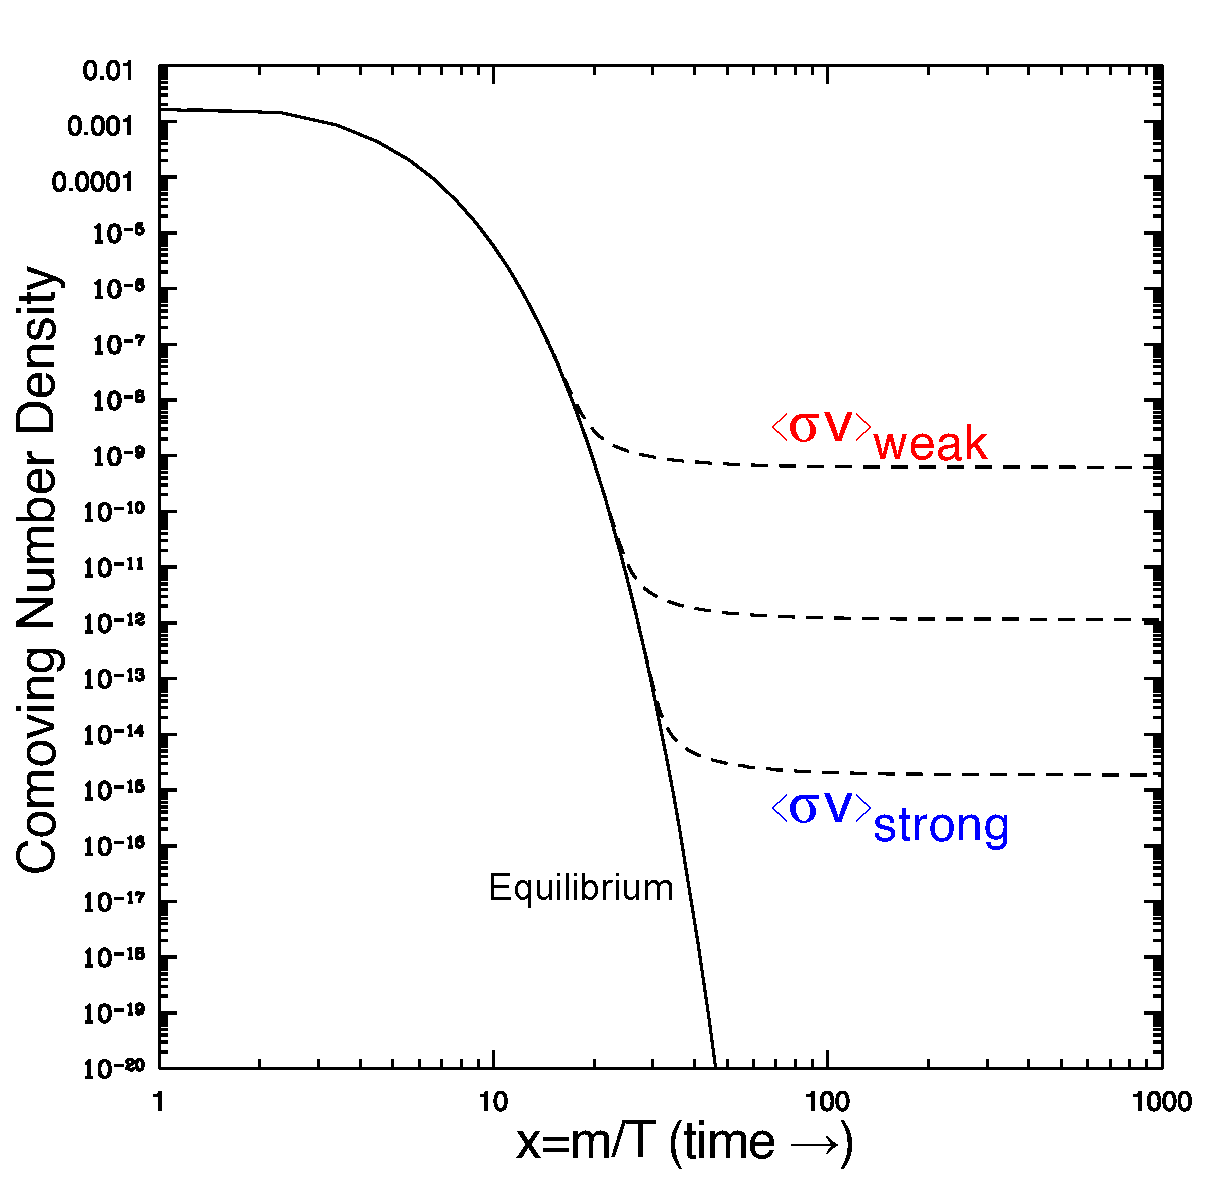
\includegraphics[width=0.65\textwidth]{chapter_01/figures/freezeout.pdf}
	\caption{\blue{Freeze-out of a thermal relic.
		The comoving abundance $Y$ is shown against the dimensionless inverse temperature $x \equiv M_\chi/T$, which grows as the Universe expands and cools.
		The solid curve is the equilibrium abundance $Y_\mathrm{eq}$, exponentially Boltzmann-suppressed once the temperature falls below the dark-matter mass ($x \gtrsim 1$).
		The dashed curves show the actual abundance for three values of the annihilation cross section: as long as annihilations outpace the Hubble expansion the abundance tracks equilibrium, and once they become inefficient it freezes out at a constant comoving value, with $Y_\infty \propto 1/\sigmav$.
		A larger cross section (lower curve) keeps the particle in equilibrium longer and leaves fewer relics than a smaller one (upper curve).
		Credit: adapted from Hooper~\cite{Hooper:2009zm}.}}
	\label{fig:freezeout_yx}
\end{figure}

\blue{Figure~\ref{fig:freezeout_yx} shows the behaviour of the solutions of Eq.~\eqref{eq:boltzmann} in these variables.}
At high temperatures \blue{the actual abundance follows the equilibrium curve $Y_\mathrm{eq}$; once the temperature drops below the rest mass, $Y_\mathrm{eq}$ collapses under the Boltzmann suppression of Eq.~\eqref{eq:neq}}.
The actual abundance tracks this decline only as long as the annihilation rate $\Gamma$ exceeds the Hubble rate $H$; once $\Gamma$ drops below $H$, annihilations can no longer keep up with expansion, $Y$ moves away from $Y_\mathrm{eq}$, and the comoving abundance plateaus at its asymptotic value $Y_\infty$.
\blue{This departure is gradual: the dark-matter abundance begins to move away from the equilibrium curve around $x \sim 10$--$15$, while the plasma is still at a temperature of order a tenth of $M_\chi$, and only settles onto its frozen plateau somewhat later.
For a weakly interacting candidate at the electroweak scale, the \emph{freeze-out} completes at $T_\mathrm{fo} \sim M_\chi/(20\text{--}25)$ --- when the particles are already non-relativistic, but the Universe is still deep in radiation domination.}

A particle that annihilates strongly enough stays in chemical equilibrium for a long time (\blue{lowest dashed curve in Figure~\ref{fig:freezeout_yx}}): it follows the equilibrium population as the latter drops exponentially, and only departs from it when the equilibrium abundance has already become small.
Such a particle leaves behind few relics.
A particle that annihilates weakly (\blue{uppermost curve}), by contrast, loses contact with the bath earlier, while its equilibrium abundance is still relatively large, and therefore freezes out at a higher residual density.
In the thermal-relic context, the weakest particle wins.
\blue{The relic abundance is thus set to first approximation by how much a candidate annihilates --- by the velocity-averaged annihilation cross section $\langle \sigma v_\mathrm{rel}\rangle$ --- while the mass enters only at second order, logarithmically, through the temperature at which decoupling occurs.}

\blue{After freeze-out both annihilation and creation become negligible, and the comoving abundance retains its plateau value $Y_\infty$; the present-day mass density in dark matter is then $\rho_\chi = M_\chi\, s_0\, Y_\infty$, with $s_0$ the entropy density today.
Dividing by the critical density gives the relic abundance
\begin{equation}
	\Omega_\chi = \frac{M_\chi\, s_0\, Y_\infty}{\rho_\mathrm{crit}}\,, \qquad \rho_\mathrm{crit} = \frac{3 H_0^2}{8\pi G}\,,
	\label{eq:omega_Y}
\end{equation}
which, evaluated with the measured entropy density and expansion rate, can be recast numerically as $Y_\infty \simeq (0.44~\mathrm{eV}/M_\chi)\,(\Omega_\chi h^2/0.12)$.
The observed abundance therefore fixes the product $M_\chi\, Y_\infty$: a heavier candidate must survive in smaller numbers to supply the same mass density.}

A subtlety worth flagging is the meaning of $\langle \sigma v_\mathrm{rel}\rangle$, since the dark-matter literature uses the term ``cross section'' for two physically distinct objects.
The $\sigma v_\mathrm{rel}$ that enters Eq.~\eqref{eq:boltzmann} (in units of cm$^3$/s) is the cross section for the process $\chi\chi \to \mathrm{SM}\,\mathrm{SM}$ multiplied by the relative velocity of the incoming pair, then averaged over a Maxwell--Boltzmann distribution at temperature $T$.
The cross section quoted in direct-detection experiments (in units of cm$^2$), by contrast, is the elastic cross section $\sigma_{\chi N}$ for the recoil process $\chi + N \to \chi + N$ on a target nucleon, involving no thermal average.
The two thus refer to different reactions, different kinematics, and different epochs in the dark-matter history.
Throughout this thesis the symbol $\langle \sigma v\rangle$ always denotes the annihilation case.
% One further point is that the relevant velocity averaging is performed at $T \sim M_\chi/25$ for freeze-out, but at $v \sim 10^{-3} c$ for indirect detection in present-day galactic halos; this mismatch motivates the velocity-dependent cases discussed in Section~\ref{sec:1.2.4}.
One further subtlety is that the thermal average entering the Boltzmann equation is evaluated at freeze-out velocities \blue{of order the thermal scale, $v_\mathrm{rel} \sim \sqrt{T_\mathrm{fo}/M_\chi} \approx 0.2\,c$}, whereas dark-matter particles in present-day galactic halos move at velocities set by the gravitational potential, $v_\mathrm{rel} \sim 10^{-3}\,c$ --- roughly two orders of magnitude smaller.
Whether $\langle \sigma v \rangle$ depends on the relative velocity therefore controls the mapping between the cosmological cross section that fixes the relic abundance and the annihilation rate accessible to indirect detection.
\blue{To keep track of this dependence we expand the annihilation cross section in partial waves, and defer its observational consequences to Section~\ref{sec:1.2.4}.}

Non-relativistic two-body annihilation admits the partial-wave expansion
\begin{equation}
	\sigma v_\mathrm{rel} \simeq \sigma_0 + \sigma_1\, v_\mathrm{rel}^2 + \mathcal{O}(v_\mathrm{rel}^4)\,,
	\label{eq:partial_wave}
\end{equation}
where $\sigma_0$ is the $s$-wave ($\ell=0$) contribution and $\sigma_1\, v_\mathrm{rel}^2$ the $p$-wave ($\ell=1$) contribution~\cite{Cirelli:2024ssz}.
\blue{Averaging this expansion over the thermal distribution of relative velocities gives $\langle \sigma v_\mathrm{rel}\rangle = \sigma_0 + (6T/M_\chi)\,\sigma_1 + \cdots$; at freeze-out, with $x_\mathrm{fo} \equiv M_\chi/T_\mathrm{fo}$, the $p$-wave term is therefore suppressed by a factor $6/x_\mathrm{fo}$ relative to the $s$-wave piece.}

\blue{Solving Eq.~\eqref{eq:boltzmann} through the freeze-out transition places the decoupling at $x_\mathrm{fo} \approx 25$, consistent with the value $T_\mathrm{fo} \sim M_\chi/(20\text{--}25)$ anticipated above; this number depends only logarithmically on the dark-matter mass and couplings, so candidates spanning a broad range of masses freeze out at comparable $x$.
The surviving comoving abundance then scales as
\[
	Y_\infty \propto \frac{x_\mathrm{fo}}{M_\mathrm{Pl}\, M_\chi\, (\sigma_0 + 3\sigma_1/x_\mathrm{fo})}\,,
\]
inversely proportional to the annihilation strength.
The $p$-wave coefficient enters here as $3\sigma_1/x_\mathrm{fo}$, rather than the $6\sigma_1/x_\mathrm{fo}$ of the instantaneous thermal average: annihilations continue to deplete the abundance after freeze-out, so the velocity-dependent term is averaged over the subsequent evolution rather than sampled at $T_\mathrm{fo}$ alone.
Inserting this into Eq.~\eqref{eq:omega_Y} yields the relic density in terms of the partial-wave coefficients~\cite{Steigman:2012nb},
\begin{equation}
	\frac{\Omega_\chi h^2}{0.12} \approx \frac{x_\mathrm{fo}}{25}\,\frac{2.2\times 10^{-26}~\mathrm{cm^3/s}}{\sigma_0 + 3\sigma_1/x_\mathrm{fo}}\,.
	\label{eq:relic_general}
\end{equation}
In the limit of pure $s$-wave annihilation the coefficient $\sigma_1$ vanishes, the thermal average becomes the constant $\langle \sigma v_\mathrm{rel}\rangle = \sigma_0$, and Eq.~\eqref{eq:relic_general} reduces, for $x_\mathrm{fo}\approx 25$, to}
\begin{equation}
	\frac{\Omega_\chi h^2}{0.12} \approx \frac{2.2 \times 10^{-26}~\mathrm{cm^3/s}}{\langle \sigma v_\mathrm{rel}\rangle}\,,
	\label{eq:relic_abundance}
\end{equation}
where the relic abundance is essentially the inverse of the annihilation cross section, with the mass entering only through logarithmic corrections to the prefactor.
The numerator is the canonical \emph{thermal cross section}, $\langle \sigma v\rangle_\mathrm{cosmo} \approx 2.2 \times 10^{-26}$~cm$^3$/s: any dark-matter candidate that annihilates at this rate reproduces, \blue{to within a few percent for masses above roughly $10$~GeV (cf.~Figure~\ref{fig:thermal_relic})}, the observed cosmological abundance.
For an annihilation amplitude characterized by a coupling $g$, with $\alpha \equiv g^2/(4\pi)$, the natural size of the cross section is $\langle \sigma v\rangle \sim \alpha^2/M_\chi^2$.
Plugging in the weak-interaction value $\alpha \sim \alpha_\mathrm{weak} \sim 0.03$ and demanding a match to $\langle \sigma v\rangle_\mathrm{cosmo}$ returns a mass $M_\chi$ of order a few hundred GeV to a few TeV --- the electroweak scale.
% , recovered without any input from particle-physics model-building.
This result is known as the \emph{\WIMP miracle}: a stable particle with mass and coupling strength at the electroweak scale, produced thermally in the early Universe, naturally yields a relic abundance consistent with the observed dark matter density~\cite{Steigman:2012nb}.
\blue{The inverse relation of Eq.~\eqref{eq:relic_abundance} is illustrated in Figure~\ref{fig:thermal_relic}: the orange band marks the cross section that reproduces the measured abundance, while smaller (larger) values freeze out too early (too late) and overproduce (underproduce) dark matter.}

\begin{figure}[t]
	\centering
	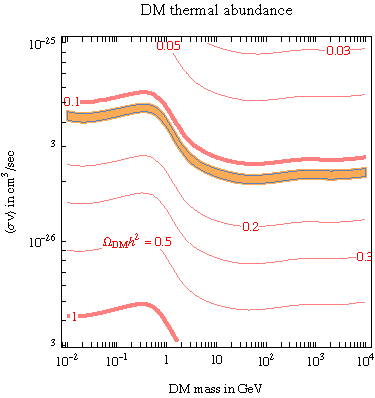
\includegraphics[width=0.47\textwidth]{chapter_01/figures/Omegafreeze-out.pdf}
	\caption{Contours for the dark matter freeze-out abundance $\Omega_\text{DM} h^2$ as a function of DM mass and annihilation cross-section $\langle \sigma v \rangle$ for Majorana dark matter.
	The measured cosmological abundance $\Omega_\text{DM} h^2 = 0.120 \pm 0.001$ is reproduced within the orange band at $3\sigma$.
	From this plot it is possible to appreciate how the annihilation cross-section needed to match the observed abundance varies with mass in the $1-3 \times 10^{-26} \, \textrm{cm}^3/\textrm{s}$ range.
	Credit: Cirelli et al.~\cite{Cirelli:2024ssz}.
	}
	\label{fig:thermal_relic}
\end{figure}

In the same $s$-wave limit, the cross section fixed by Eq.~\eqref{eq:relic_abundance} also sets the rate at which dark matter annihilates in present-day astrophysical environments.
This connection between cosmological abundance and indirect-detection signals further motivates the gamma-ray searches of Chapters~\ref{ch:4}--\ref{ch:8}.
